\documentclass{beamer}
\usepackage[utf8]{inputenc}

\usetheme{Boadilla}
\usecolortheme{default}


\usepackage[T2A]{fontenc}
\usepackage[utf8]{inputenc}

\hypersetup{
    colorlinks=true,
    linkcolor=blue,
    filecolor=magenta,      
    urlcolor=cyan,
    pdftitle={Overleaf Example},
    pdfpagemode=FullScreen,
    }

\title[Introduction to LaTeX] 
{History of Intel}

\author[Tyuplyaev] 
{N.~A.~Tyuplyaev\inst{1}}

\institute[HSE] 
{
  \inst{1}
  Faculty of Computer Science \\
  HSE University
}

\date[July 2022] 
{LaTeX Course, July 2022}

\logo{
\includegraphics[height=1cm]{img/logo.png}}    

\AtBeginSection[]
{
  \begin{frame}
    \frametitle{Table of Contents}
    \tableofcontents[currentsection]
  \end{frame}
}


\begin{document}

\frame{\titlepage}

\begin{frame}
\frametitle{Table of Contents}
\tableofcontents
\end{frame}


\section{Intro}

\begin{frame}
\frametitle{Intro}
\begin{block}{Brief introduction of the company}
Intel, in full Intel Corporation, American manufacturer of semiconductor computer circuits. It is headquartered in Santa Clara, California. The company’s name comes from “integrated electronics.” For nearly 40 years, Intel Corporation has been at the forefront of silicon innovation. Today it is the world leader in developing technologies, products, and initiatives to continually advance how people work and live.
\end{block}
\end{frame}

\section{Beginnings}

\begin{frame}
\begin{block}{Brand foundation}
Intel was founded in July 1968 by American engineers Robert Noyce and Gordon Moore. Unlike the archetypal Silicon Valley start-up business with its fabled origins in a youthful founder’s garage, Intel opened its doors with 2.5 dollars million in funding arranged by Arthur Rock, the American financier who coined the term venture capitalist. Intel’s founders were experienced, middle-aged technologists who had established reputations. Noyce was the coinventor in 1959 of the silicon integrated circuit when he was general manager of Fairchild Semiconductor, a division of Fairchild Camera and Instrument. Moore was the head of research and development at Fairchild Semiconductor. Immediately after founding Intel, Noyce and Moore recruited other Fairchild employees, including Hungarian-born American businessman Andrew Grove. Noyce, Moore, and Grove served as chairman and chief executive officer (CEO) in succession during the first three decades of the company’s history.
\end{block}
\end{frame}

\begin{frame}{Early products}
\begin{center}
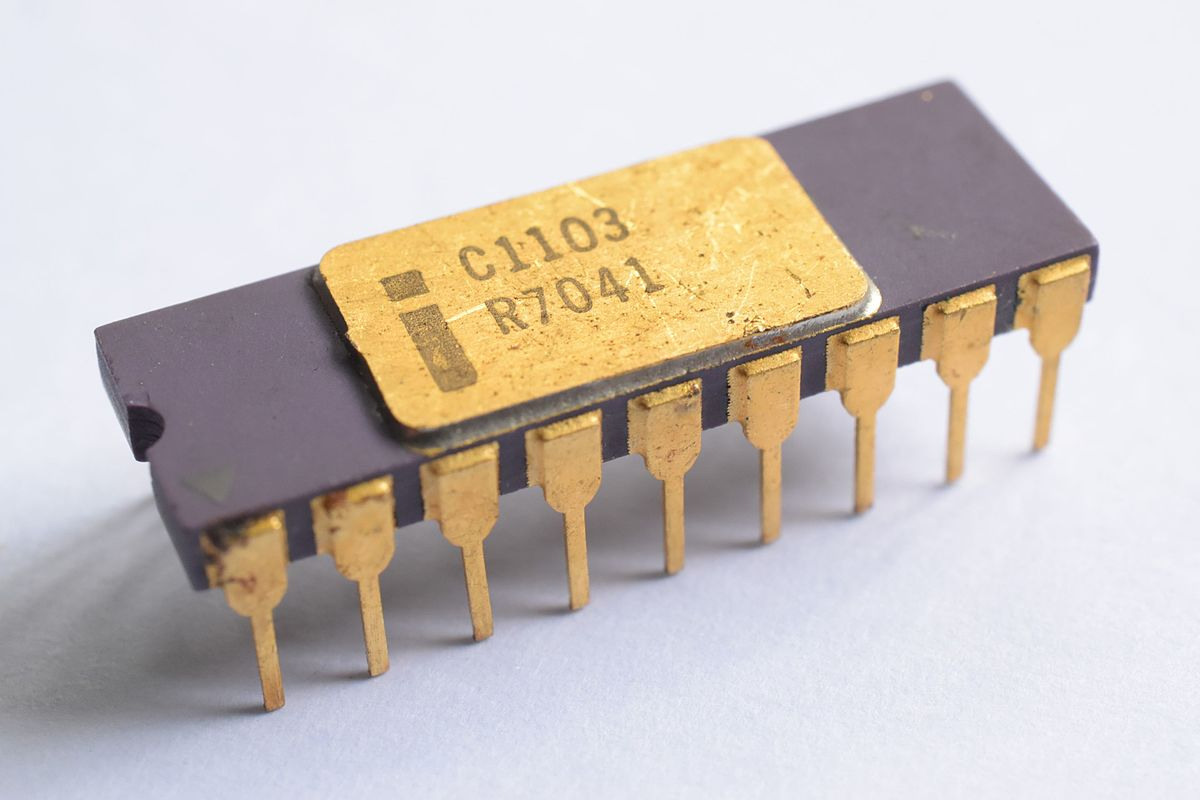
\includegraphics[width=.3\linewidth, height = 3 cm]{img/dram.jpg}\quad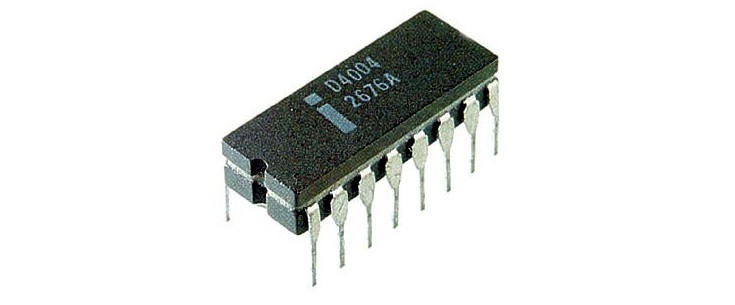
\includegraphics[width=.3\linewidth, height = 3 cm]{img/cpu.jpg}\quad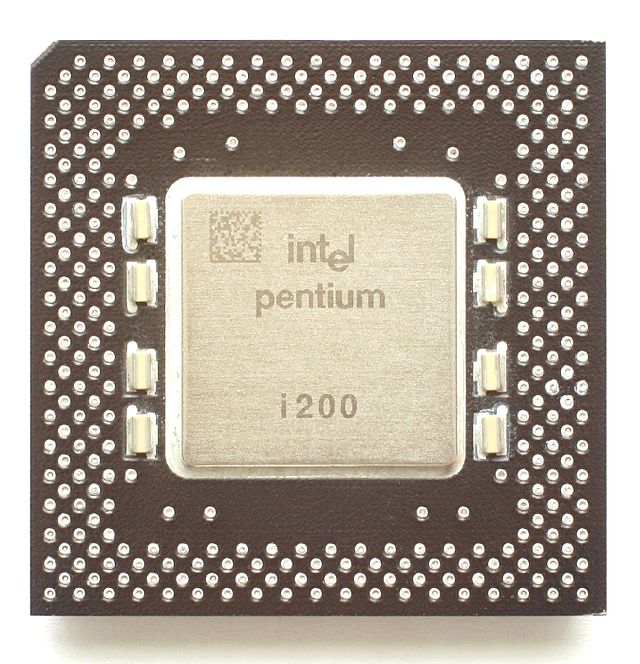
\includegraphics[width=.3\linewidth, height = 3 cm]{img/pentium.jpg} 
\\[\baselineskip]
\end{center}
Intel's fist DRAM, microprocessor and the first one Pentium processor 
\end{frame}

\begin{frame}
\begin{block}{Pentium processor}
With the introduction of the Pentium microprocessor in 1993, Intel left behind its number-oriented product naming conventions for trademarked names for its microprocessors. The Pentium was the first Intel chip for PCs to use parallel, or superscalar, processing, which significantly increased its speed. It had 3.1 million transistors, compared with the 1.2 million transistors of its predecessor, the 80486. Combined with Microsoft’s Windows 3.x operating system, the much faster Pentium chip helped spur significant expansion of the PC market. Although businesses still bought most PCs, the higher-performance Pentium machines made it possible for consumers to use PCs for multimedia graphical applications such as games that required more processing power. 
\end{block}
\end{frame}

\section{Modern History and Products}

\begin{frame}
\begin{block}{Expansion and other developments}
In January 2006, the company announced it had designed what is believed to be the first fully functional SRAM (static random access memory) chip using 45-nanometer (nm) logic technology. Then, just a year later, Intel began to implement an innovative combination of materials that drastically reduced transistor leakage, improving energy efficiency, and significantly increasing performance in its 45nm process technology. Intel now uses a new material based on the element hafnium instead of silicon with a property called “high-k” for its transistor gate dialectric, and a new combination of metals for the transistor gate in portions of the millions of transistors inside a multi-core computer chip, which is about the size of a postage stamp. Paul Otellini succeeded Barrett as Intel’s CEO in 2005, and four years later Jane Shaw replaced Barrett as chairman. She held the post until 2012, when she was succeeded by Andy Bryant. The following year Brian Krzanich became CEO. In 2019 chief financial officer Bob Swan became CEO, and Intel ranked 43 on the Fortune 500 list of the largest American companies.
\end{block}
\end{frame}

\begin{frame}
\textbf{Nowadays the following products are manufactured by Intel:}
\begin{itemize}
    \item The 8-bit processors
    \item The 16-bit processors
    \item The 32-bit processors
    \item The 64-bit processors
    \item Microcontrollers
    \item 7-9th generation Core
    \item 10th generation Core
    \item 11th generation Core
    \item 12th generation Core
\end{itemize}
\end{frame}

\begin{frame}{Some images if Intel's modern products}
\begin{center}
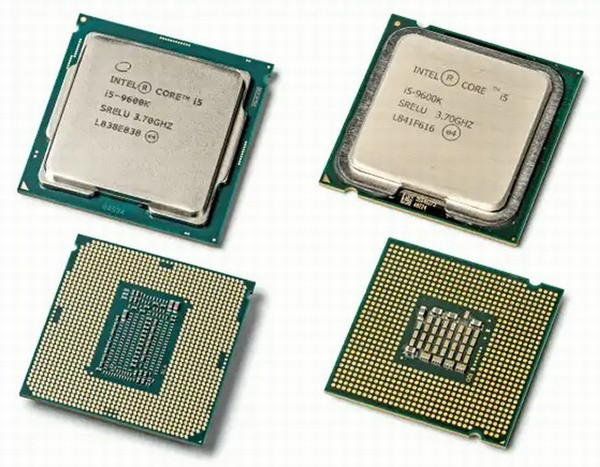
\includegraphics[width=.3\linewidth, height = 4 cm]{img/a.jpg}\quad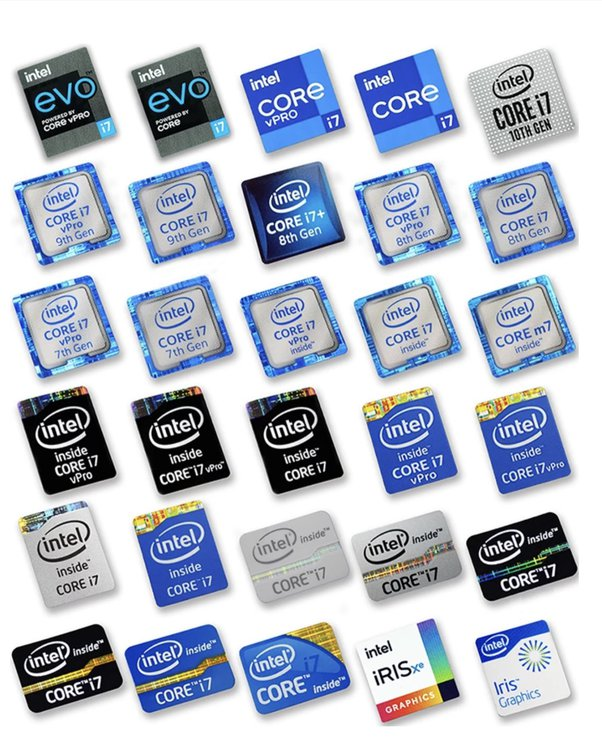
\includegraphics[width=.3\linewidth, height = 4 cm]{img/b.jpeg}\quad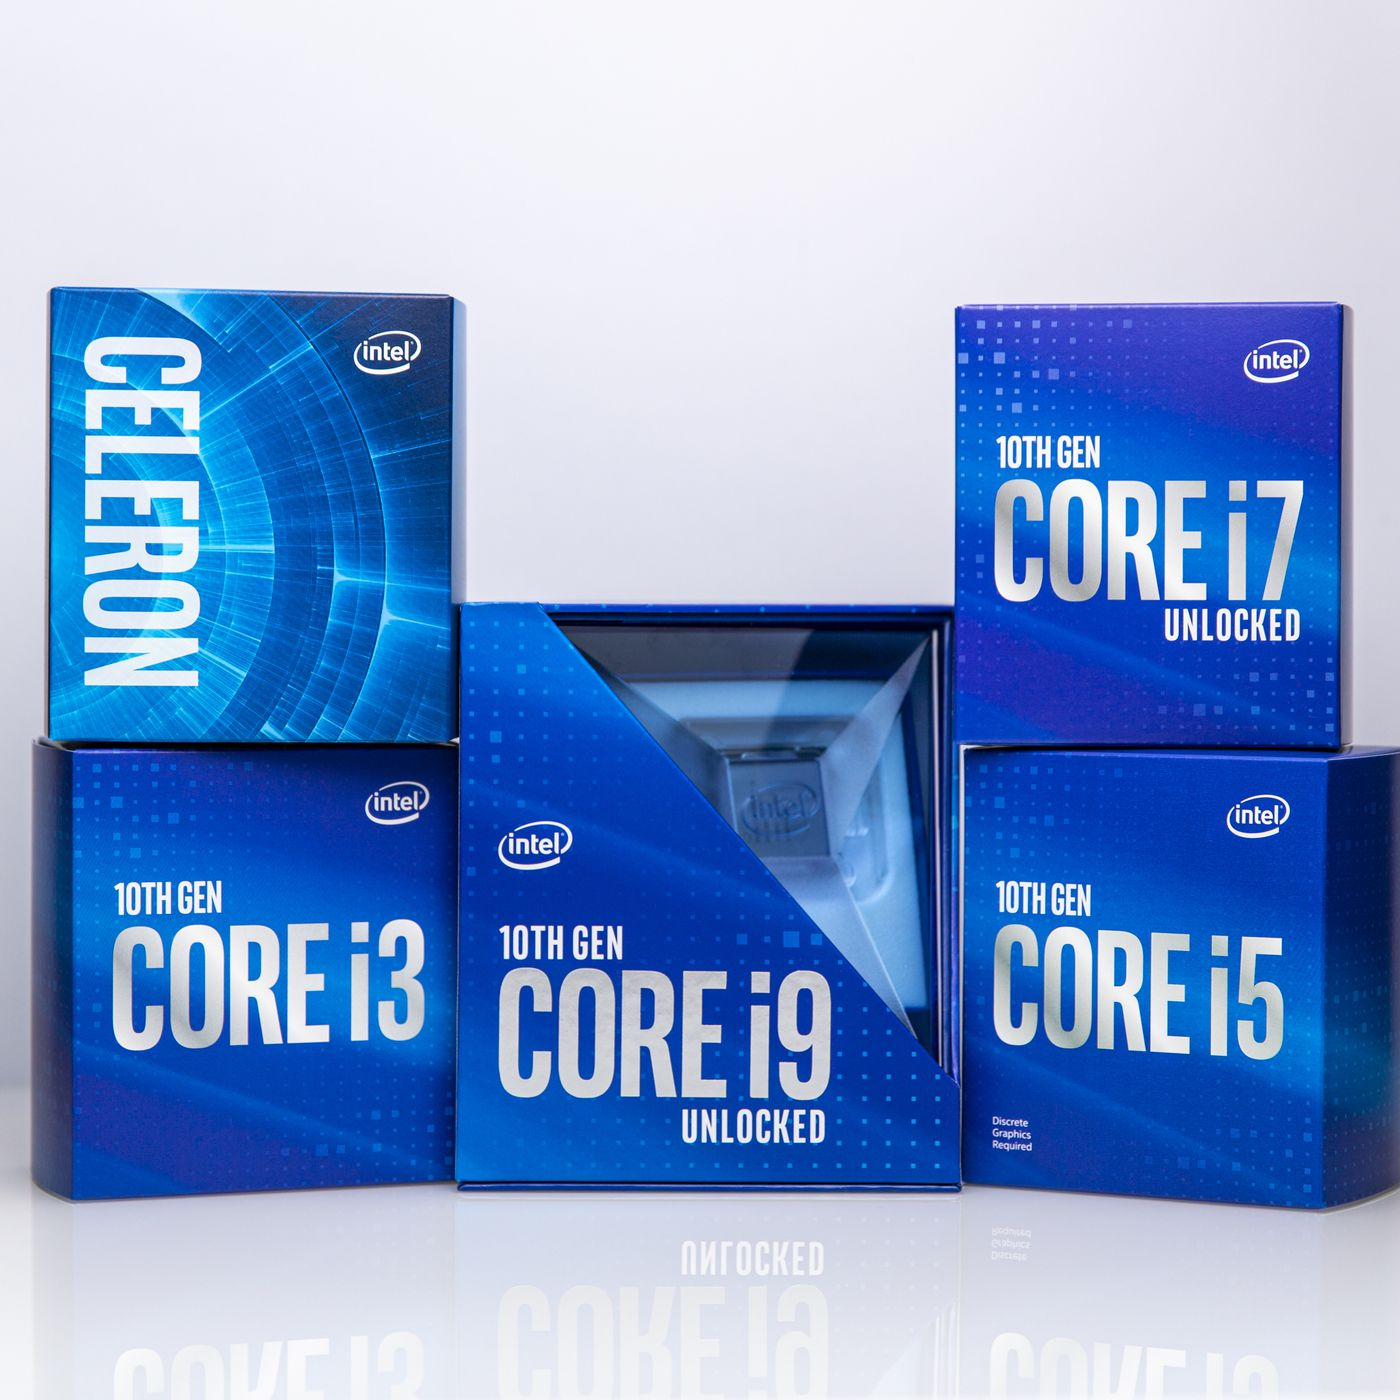
\includegraphics[width=.3\linewidth, height = 4 cm]{img/c.jpg} 
\\[\baselineskip]
\end{center}
\end{frame}

\begin{frame}
\huge\textbf{Thank you for attention!}
\end{frame}





\end{document}